\section{Solution}\label{solution}

%2.5 pages
%Renan: Solucao-Intro
%Renan: Solucao-Manipulator
%Estevão: Solucao-Rails (Renan revision)
%Estevão/Renan: Solucao-Shutter
%TODO Gabriel: Solucao-Calibration

Regarding the environment constraints detailed in Sec.~\ref{problem}, the
conceptual solution of EMMA is a mid-sized robotic manipulator with a modular
rail base. As the manipulator can not fully cover the blade surface in a
fixed position, and the robot locomotion is complex in the turbine's
environment, a customized rail should provide extra degrees of freedom (DOF) to
the system. EMMA aims to be a generic solution to bulb turbines, being modular,
and versatile. It is an autonomous system for hard coating applications, thus
the following system's elements will be presented: the robotic manipulator; the
customized base; and the robot calibration.


\subsection{Robotic Manipulator}\label{manipulator}
Trying to propose an \textit{in situ} turbine hard coating solution similar to
the \textit{ex situ} solution is a natural thought. Therefore, the first step of
EMMA's development was the research for industrial robotic manipulators. The
compilation of the HVOF coating requirements and environment constraints demands
a mid-sized robotic manipulator, as a large-sized one would not be able to move
inside the confined space and would not fit at the back side of the
runner's blade, and a small-sized one would not have the required payload and
speed for the process. In EMMA's project, the robotic manipulator will be
responsible for the coating application, precision, and tool handling.

A market survey was conducted to determine the most suitable industrial robotic
manipulator for the application. A 3D CAD model of the hydropower turbine was
built, and overall simu\-lations and analysis were performed using the Open
Robotics Automation Virtual Environment (OpenRave) \cite{diankov2008openrave}.
The simulations involve runner's blade discretization, coating strategy,
coating segmentation (partitioning) and base positions computation for full
blade cover, and robotic manipulator kinematics and dynamics. Among the
analyzed mid-sized robotic manipulators, the Yaskawa Motoman MH12\raisebox{1ex}{\textregistered}
robot was chosen due to its satisfactory workspace, and versatility.

To achieve a good coating quality, the HVOF process requires that the robotic
manipulator's end-effector moves with a constant 40~m/min speed along the
blade's surface. The typical path of HVOF coating is a zigzagging trajectory,
i.e., it is a deceleration/acceleration process with direction changes. As the
\textit{ex situ} solution uses a large-sized robotic manipulator, the
end-effector's direction changes occur outside the blade's range, complying the
speed requirement in the blade's range. However, while deceleration or
acceleration, coating material is wasted to the environment or, most commonly
to a shadow plate.

The mid-sized robot for \textit{in situ} operation makes this strategy
impossible, as, at some base positions, the robot will always be in the blade's
range. The proposed solution modifies the original circuit of the gases that
carry the coating particles to a new 2-way controlled circuit, in wich there is a directional
valve that changes the flow path from the thermal spray gun to return to tank
circuit. %TODO Estevao: figura do processo
The directional valve is autonomously actuated accordingly to the robotic
manipulator's trajectory, i.e., the valve will ``shut'' while end-effector's
direction changes. Therefore, the solution provides coating material savings,
as the non-used particles are stored for future usage, and the hard coating
speed requirement is met.

\begin{figure}[h!]
   \centering
   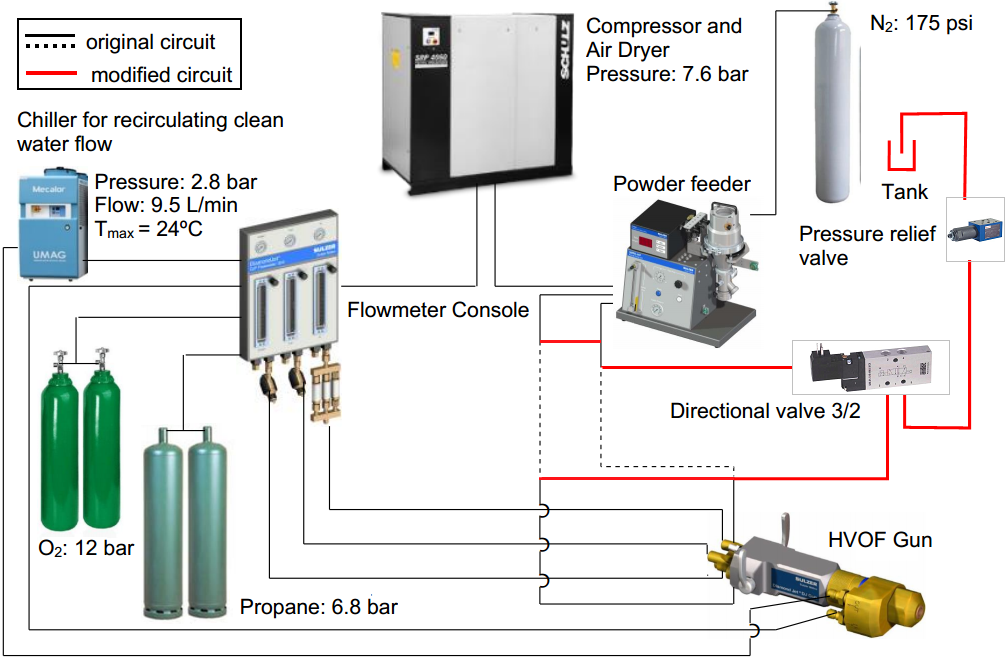
\includegraphics[width=0.9\columnwidth]{figs/mecanica/Circuito_HVOF_mod_en.PNG}
   \caption{Simplified view of HVOF circuit with shutter}
   \label{fig::circuito_hvof}
\end{figure}

Despite being able to coat approximately 50\% of the blade on a fixed
position, kinematic and dynamic analysis show that the MH12 robot can not fully
cover it vertically or horizontally, demanding 2-DOF along the blade's surface.
The coating strategy and blade coating partitioning reveal that the blade's top
extremities require an specific base position, reachable
with a primary rail between the blades. Therefore, the MH12 robot will require
at least four positions along the blade and one position on a primary
rail, between blades. 

\subsection{Base}
% 0.75 pages

EMMA's base comprises two rails, forming two prismatic joints. The
first, or primary rail, is parallel to the turbine axis, and it is responsible
for the transportation of the robotic manipulator between the hatch and the
blade. The secondary rail is is parallel to the blade's surface, and it is
assembled from the first rail by a rotational joint for angle adjustment. A
third prismatic joint is placed in the secondary rail for height adjustment of
the robotic manipulator. These rails guarantee the full coating cover, as they
allow the robotic manipulator movement in the confined space, by a 4-DOF
base, Prismatic-Rotational-Prismatic-Prismatic (PRPP) joints. 
%TODO Estevao: colocar figura

The hatch limits the size of the rail in terms of weight and geometry, thus a
modular concept was design, such that the small modular parts can be easily and
manually assembled inside the turbine. The base is a modular two parallel
profiled rail system %TODO Estevao: colocar referencia
with a four carriage setup. In this configuration, the reaction moments of the
base are cancelled by a force couple provided by each couple of carriages. The
% and the loads are divided in ore components.
%TODO Estevao: colocar figura
commercial modules are aluminum structures for corrosion resistance,
lightweight, geometric flexibility, and modularity, as it is possible to
increase/decrease the rail length/width/height by changing few parts or adding
anchor arms. %TODO Estevao: referencia para as propriedades do aluminio
% (aplicacao)

The resulting base is a slender and lightweight frame, such that a careful
analysis is necessary to evaluate the structural integrity and rigidity, in
respect to the dynamic loads of the robotic manipulator. A Finite Element
Analysis (FEA) was performed to study the stresses, strains and resultant forces
along the structure. FEA is also used to size the frame components, such as
the profile's size, and to size the anchors, its directions, and attachment to
provide the greater base's rigidity. The rigidity is a major concern, it is
required for the hard coating process, since a non-rigid base propagates
vibrations to the robotic manipulator's end-effector with high amplitudes, which
may compromise coating quality.
%TODO Estevao: qual o software do FEA?

The draft tube and runner area are conical shape structures, curved and
sloped. The environment modification, as wielding and drilling, should be
avoided, thus properly fixing the base on the ground is a major challenge in
EMMA project. The draft tube is composed of a ferromagnetic steel material,
hence magnetic fixtures may be suitable for base attachment. 

Common magnetic fixture products are temporary magnetic equipments used to hoist
and transport materials in an industrial plant. In EMMA, it is used to attach
and anchor the rail's modules to the ground. Field tests were conducted in the
draft tube for payload evaluation, at different equipment's orientations. The
results concluded that the magnetic fixture is sufficient for this application.
%TODO Estevao: resumir o teste que foi feito em uma frase dentro deste
% parágrafo. Colocar qual o dispositivo selecionado.

\subsection{Calibration}

In opposition to \textit{ex situ} operations, in which the relative position
between the robot and the blade to be coated is fixed, \textit{in situ}
operation requires robot and blade localization and pose. In EMMA's context,
system calibration is robot and blade identification, and pose estimatation in
respect to the environment. To gather tridimensional information about the
turbine's environment, a laser scanner is placed inside the hydraulic circuit
and the pose estimation is divided in: robot localization, and
localization of the blade.
 
The attachment of markers on the manipulator or its base can be performed with
precision and repeatability, thus reflective spheres were choosen to serve
as reference in the process of localization of the manipulator in respect to the
environment. These spheres are indetified inside the point cloud by a 3D Hough
transform method based on the work of \cite{camurri20143d}. The 3D Hough
transform, as its two dimensional counterpart, is a search on the (discretized)
parametric space of the object. A sphere has a four dimensional parameter space, tree for
the position of its center and one for its radius. For each point on the point
cloud, it is assined a collection of points on the discretized parametric space
(corresponding to the viable spheres passing through that point). Those points
of the discretized parametric space which have a great number of point assined
to are probable spheres. There might arise issues on the size of the parameter
space, but it is reduced by previous knowledge on the expected radius of the
spheres and viable region for the robot inside the enviroment.

The pose estimation of the blade cannot be assisted with the introduction of
markers, and the localization process must rely only on the intrinsec properties
of the blade's surface geometry. As proposed in \cite{Tombari2010a}, a point
cloud model of the blade is compared to the point cloud of the scene aquired by
the laser sensor. A subset of points in each point cloud is enhanced with a
local description of its local neighborhood. Given the sets of features, it is
possible to determine the correspondence between the two sets. If enough
correspondences are found in the scene, above a threshold, the blade is
identified and the position is determined by the correspondences.
%TODO Abelha: o que é mapear e calibrar no contexto do EMMA? Como é feita a
% calibração e o mapeamento, quais os sensores? quais os algoritmos?
